\documentclass[11pt]{article}
\usepackage[T1]{fontenc}
\usepackage{graphicx}
\usepackage{lmodern}
\usepackage{multicol}
\usepackage{enumitem} 
\usepackage[margin=0.85in]{geometry}
\usepackage{amsmath,amssymb}
\usepackage{setspace}
\usepackage{float}
\usepackage{subcaption} 
\usepackage[backend=bibtex,style=ieee]{biblatex}
\usepackage{siunitx} % units and angles

% tighten figure–equation spacing
\setlength{\textfloatsep}{6pt plus 1pt minus 1pt}
\setlength{\intextsep}{6pt plus 1pt minus 1pt}
\setlength{\abovecaptionskip}{1pt}
\setlength{\belowcaptionskip}{0pt}

\addbibresource{sources.bib}


\title{Midtern Project: Supersonic Train Design}
\author{Sophia Klymchuk \\
\small Prof. Chacon \\ 
\small ME-433: Rocket Science}


\begin{document}
\maketitle

\section{Introduction}

The objective of this project is to design the front-end shape of a supersonic train that minimizes total operating cost while remaining within the prescribed physical and aerodynamic constraints. The train’s nose shape must fit entirely within a square bounding box of side length $L = \SI{1}{\meter}$, with a constant depth of $\SI{1}{\meter}$ into the page.

The system operates in a supersonic flow entering from the left, under the following freestream conditions:
\[
M = 3, \quad T = \SI{300}{\kelvin}, \quad P = \SI{101{,}325}{\pascal}
\]

The goal is to minimize the cost function $C = 20ND$, where $N$ is the number of trips required to transport a total payload of $\SI{1}{\meter^3}$, and $D$ is the total drag force acting on the train’s front-end design.

To calculate drag, we utilize two separate physical flow models: an inviscid and a viscous case. For both cases, the pressure at the back face $AB$ is assumed to be a vacuum.

Only oblique shocks and expansion waves are considered in the flow model. The analysis thus mandates that the turning angles of all surface segments remain within the valid range for attached oblique shocks.

The performance metric is based solely on horizontal drag. The payload volume and number of trips $N$ are determined by the enclosed area of each 2D train profile, since the depth is constant. The design that achieves the lowest cost $C$ under these physical constraints is considered optimal.

It should be noted that for the working fluid of air in this project, we make the Ideal Gas and the Calorically Perfect Gas assumptions, as well as assumptions of steady, 1D flow. The ratio of specific heats is taken to be $\gamma_{air}=1.4$.

\section{The Cost Function}
To evaluate the fitness of each shape, we are presented with a cost function to minimize, which is displayed in Equation \ref{eq:cost_func}. In this equation, $N$ represents the number of trips the train would need to take in order to transport $\SI{1}{\meter^3}$ (the total volume of the bounding box) of payload from one city to another. $D$ represents the total drag of the design.
\begin{equation}
C = 20 N D
\label{eq:cost_func}
\end{equation} 
\subsection{Number of Trips}
Because each train shape is generated as a constant-depth 2D profile with a depth of $\SI{1}{\meter}$ into the page, the volume ratio between the train and the bounding box can be represented equivalently as an area ratio.

If a profile encloses an area of $\SI{0.5}{\meter^2}$, this corresponds to half the total bounding box volume. The train would therefore require two outbound trips to transport the full payload, plus one return trip to reload, for a total of three trips. Via intuition, we can recognize that the formula for such a behavior emerges as displayed in Equation \ref{eq:num_trips}.
\begin{equation}
N = 2 \text{ ceiling}\left(\frac{\SI{1}{\meter^3}}{A_{profile}}\right)-1
\label{eq:num_trips}
\end{equation} 
The area of each profile is calculated via a simple difference of the Trapezoidal Rule applied to the top and bottom sides of the profile.

\subsection{Drag}
Firstly, drag calculations for the cost are split into two physical models:
\begin{enumerate}
    \item Inviscid Assumption: With the assumption of no fluid viscosity, there is no friction / "no-slip conditions" at the profile surfaces. Thus, all drag is pressure drag.
    \item Viscous Case: When we drop the assumption of an inviscid fluid, drag on the profile surfaces becomes the sum of pressure drag as well as skin drag at the surface boundary.
\end{enumerate}
Drag calculations are done in a manner similar to Problem 3 of Homework 4. Given a set of top and bottom profile points, we find the surface angles at each corner with respect to the global horizontal axis (see Equation \ref{eq:surface_angle}). The difference between consecutive surface orientations gives the turn angles (see Equation \ref{eq:turn_angle}), which define whether the local flow experiences an oblique shock (positive turn angle) or an expansion wave (negative turn angle).
\begin{equation}
\theta_{surface}=\tan^{-1}\left( \frac{y_{i+1}-y{i}}{x_{i+1}-x_i}\right) 
\label{eq:surface_angle}
\end{equation}
\begin{equation}
\theta_{turn}=
\begin{cases}
\theta_{sur, i+1}-\theta_{sur, i}, \quad \text{top surface}\\
\theta_{sur, i}-\theta_{sur, i+1}, \quad \text{bottom surface}
\end{cases}
\label{eq:turn_angle}
\end{equation}

From these turn angles, the local Mach number, pressure, density, and temperature ratios are computed sequentially using either oblique-shock (see Equation \ref{eq:oblique_shock}) or Prandtl–Meyer and isentropic expansion relations. Note that for oblique shocks, the shock angle $\beta$ which is used in many of these calculations is found from the Theta-Beta-Mach Relation, which can be seen in Equation \ref{eq:tbm}.
\begin{subequations}
\begin{align}
M_{n1} &= M_1 \sin \beta \\[6pt]
\frac{\rho_2}{\rho_1} &= \frac{(\gamma + 1) M_{n1}^2}{(\gamma - 1) M_{n1}^2 + 2} \\[6pt]
\frac{p_2}{p_1} &= 1 + \frac{2 \gamma}{\gamma + 1} (M_{n1}^2 - 1) \\[6pt]
M_{n2}^2 &= \frac{M_{n1}^2 + \dfrac{2}{\gamma - 1}}{\dfrac{2 \gamma}{\gamma - 1} M_{n1}^2 - 1} \\[6pt]
\frac{T_2}{T_1} &= \frac{p_2 \rho_1}{p_1 \rho_2} \\[6pt]
M_2 &= \frac{M_{n2}}{\sin(\beta - \theta)}
\end{align}
\label{eq:oblique_shock}
\end{subequations}
The Prandtl-Meyer relations are shown in Equation \ref{eq:prandtl_meyer}, and the isentropic stagnation state equations are displayed in Equation \ref{eq:isentropic}. Since expansion waves are isentropic processes, the stagnation state of the flow before and after the wave will be equal, which allows us to relate latter to former state. The choice of which relation to use is via the sign of the turn angle. These ratios are then converted to absolute values using the given freestream properties of Mach number, static pressure, and temperature. Density is obtained from the ideal gas law.
\begin{equation}
\nu(M) = 
\sqrt{\frac{\gamma + 1}{\gamma - 1}} 
\tan^{-1} \!\left[
\sqrt{\frac{\gamma - 1}{\gamma + 1} (M^2 - 1)}
\right] - \tan^{-1} \!\left[ \sqrt{M^2 - 1} \right]
\label{eq:prandtl_meyer}
\end{equation}

\begin{subequations}
\begin{align}
a &= \sqrt{\gamma R T} \\
\frac{p}{p_0} &= \left( 1 + \frac{\gamma - 1}{2} M^2 \right)^{-\frac{\gamma}{\gamma - 1}} \\
\frac{T}{T_0} &= \left( 1 + \frac{\gamma - 1}{2} M^2 \right)^{-1}\\
\frac{\rho}{\rho_0} &= \left( 1 + \frac{\gamma - 1}{2} M^2 \right)^{-\frac{1}{\gamma - 1}} 
\end{align}
\label{eq:isentropic}
\end{subequations}

Once we have the absolute values at each face of the profile, we find pressure drag via summing up the component of pressure acting parallel to the flow, multiplied by the length of the face segment, as well as the depth into the page (given as $1$ m). To find skin drag, we utilize Equation \ref{eq:skin_drag}, where the drag coefficient is given as $C_D=0.01$, the area is face-segment length multiplied by depth into the page, and the density and velocity are those of the fluid touching the subsection (found as explained in the previous paragraph). It should be noted that we multiply the assignment's given equation by the $\cos(\theta_{surface})$ term in order to get the viscous drag component along the direction of fluid flow (which is the same direction as the pressure drag). The drag is calculated at each face of each profile, and then summed up to give a total drag for the profile.
\begin{equation}
    D=\frac{1}{2} \rho v^2 C_D A \cos(\theta_{surface})
    \label{eq:skin_drag}
\end{equation} 

It should be noted that there will be certain profiles for which, when we calculate drag, flow conditions will violate model assumptions. For example, turn angles may exceed maximum oblique-shock limits (thus forcing a detached shock), or flow may fall below supersonic Mach values. The oblique-shock limit of $\theta_{max}$ is calculated via numerical analysis of the Theta-Beta-Mach Relation (see Equation \ref{eq:tbm}), and these cases are identified and marked with an infinite cost as to disqualify them from further consideration in the design space.
\begin{equation}
\tan \theta = 2 \cot \beta 
\left[
\frac{M_1^2 \sin^2 \beta - 1}
     {M_1^2 (\gamma + \cos 2\beta) + 2}
\right]
\label{eq:tbm}
\end{equation}


\section{Shape Generation}
For all shapes generated, we assume a single starting point at which the top and bottom surfaces meet. This point was chosen to be at the left-hand side of the bounding box, positioned at $P_{start}=(0,0.5)$. This was done because:
\begin{enumerate}
    \item A shape that does not face the incoming flow with a single point, but rather a flat face, would experience significant pressure drag because the incoming supersonic flow would act directly on a surface oriented normal to the flow direction. While it is arguable that these shapes could be generated and then simply evaluated for their costs, I made the decision after some preliminary testing that none of these shapes would be favorable due to their large upfront drag cost. Excluding them from the design space improves the speed and focus of the optimization process without sacrificing viable solutions.
    \item While it is possible to start the shape from a point located in the middle of the bounding box (such as a $(0.5,0.5)$ starting point), these configurations provide no meaningful advantage. Any such geometry can be equivalently represented by shifting the shape to begin at the left boundary and extending its rear surface horizontally. This horizontal extension increases the volume and therefore reduces the number of required trips without affecting the pressure drag in the inviscid case, since all extra these horizontal surfaces are parallel to the flow direction. In the viscous case, this modification only slightly increases skin friction drag due to the larger wetted area, a minor tradeoff compared to the volumetric benefit. Additionally, shapes that expand outward from a central starting point would have to adopt steeper surface slopes to enclose the same internal volume as the same shape starting at $x=0$. In most cases, these slopes exceed the maximum allowable deflection angle for an oblique shock at the leading edge, resulting in invalid oblique shock flow behavior (as the shock would detach) and increased drag (as those faces would have a greater area component normal to incoming flow).
\end{enumerate}
All shapes generated via code are returned as 3 lists: x-values, top surface y-values, and bottom surface y-values.


\subsection{Parabolic Profile}
The parabolic shape is generated according to Equation \ref{eq:parabola}, where $a$ is the curvature parameter controlling the vertical spread of the profile. An example can be seen in Figure \ref{fig:parabola}.
\begin{subequations} \label{eq:parabola}
\begin{align}
y_{\text{top}} &= a\sqrt{x} + 0.5 \label{eq:parabola_top}\\
y_{\text{bot}} &= -a\sqrt{x} + 0.5 \label{eq:parabola_bot}
\end{align}
\end{subequations}
Higher $a$ values produce blunter shapes with wider cross-sections, while smaller values yield sharper, more streamlined noses. Both surfaces are clipped to remain within $y \in [0,1]$. The number of discrete points $N$ (default 100) determines spatial resolution, and also contributes to the sharpness or bluntness of the parabola (since a lower resolution will approach a more polygonal shape, rather than curved).
\begin{figure}[H]
\centering
    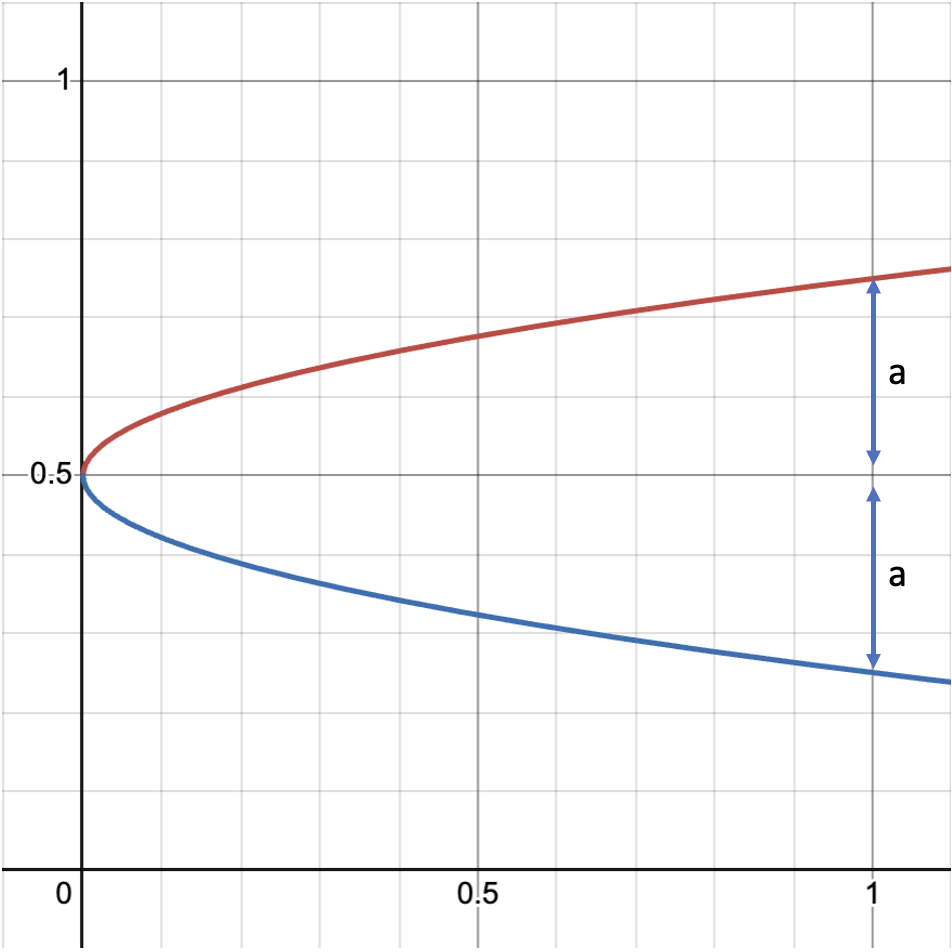
\includegraphics[width=0.5\linewidth]{parabola.png}
    \caption{Parabola profile with the spread parameter $a$ marked.}
\label{fig:parabola}
\end{figure}

\subsection{Power Series Profile}
The power-series profile generalizes the parabolic shape using a power-law dependence on $x^{0.66}$, as given in Equation~\ref{eq:power_series}. The single parameter $h_{\text{base}}$ controls the vertical amplitude. Figure \ref{fig:power} provides an example profile.
\begin{subequations} \label{eq:power_series}
\begin{align}
y_{\text{top}} &= h_{\text{base}}\,x^{0.66} + 0.5 \label{eq:power_series_top}\\
y_{\text{bot}} &= -h_{\text{base}}\,x^{0.66} + 0.5 \label{eq:power_series_bot}
\end{align}
\end{subequations}
This formulation produces a smoother curvature near the nose compared to the parabolic profile, with a gradual widening toward the rear. The function is typically sampled with $N = 100$ evenly spaced points. It should be noted that this profile's equation was utilized due to its mention by Kumar et. al as the optimal choice for ViPER class rockets operating at at least Mach-2 \cite{gDesignCFDAnalysis2020}.
\begin{figure}[H]
\centering
    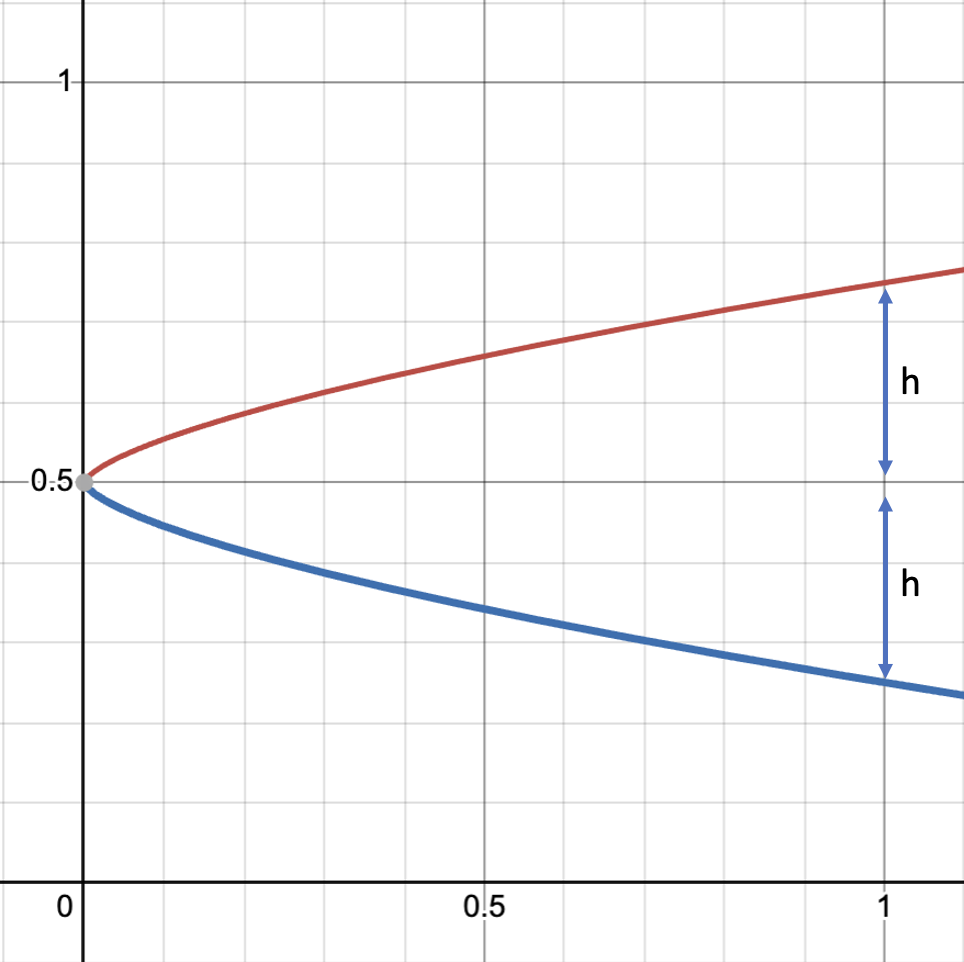
\includegraphics[width=0.5\linewidth]{power.png}
    \caption{Power series profile with the base height parameter $h$ marked.}
\label{fig:power}
\end{figure}


\subsection{Triangular Profile}
The triangular profile is defined by a single geometric parameter, the inner half-angle $\theta$, which determines the slope of the linear surfaces as shown in Equation \ref{eq:triangle_slope}. An example triangle is shown in Figure \ref{fig:triangle-a}.
\begin{equation}
m = \tan\!\left(\theta\right)
\label{eq:triangle_slope}
\end{equation}
The upper and lower surfaces extend linearly from the starting point $(x,y) = (0,0.5)$ until either reaching the top or bottom boundaries or the end of the bounding box at $x = 1$. If clipping occurs before $x = 1$, a rectangular section is appended to maintain full length (see Figure \ref{fig:triangle-b}). This shape produces a minimal, pointed leading edge. 
\begin{figure}[H]
\centering
\begin{subfigure}[b]{0.45\textwidth}
    \centering
    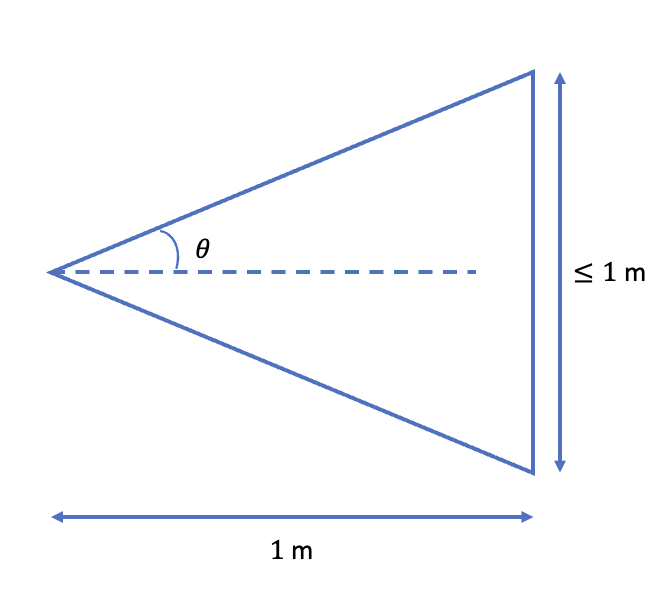
\includegraphics[width=\linewidth]{triangle_a.png}
    \caption{Triangle profile without clipping.}
    \label{fig:triangle-a}
\end{subfigure}
\hfill
\begin{subfigure}[b]{0.45\textwidth}
    \centering
    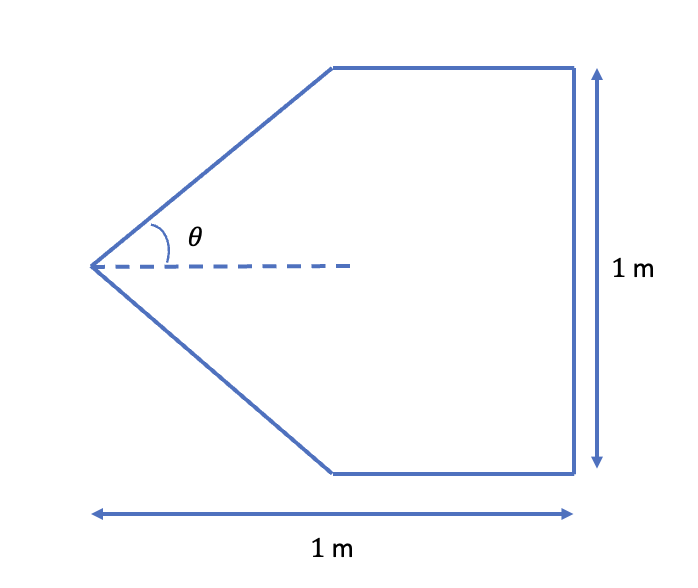
\includegraphics[width=\linewidth]{triangle_b.png}
    \caption{Triangle profile clipped to fit in $y \in [0,1]$.}
    \label{fig:triangle-b}
\end{subfigure}
\caption{Triangle profiles with the inner half-angle $\theta$ marked}
\label{fig:triangle}
\end{figure}

\subsection{Triangular Wedge Profile}
The triangular wedge introduces an additional base height parameter $h_{\text{base}}$ to control the vertical extent of the rectangular region behind the wedge, so this class produces triangles similar to the clipped triangles, but with more control over their total height. The top and bottom bounds are defined in Equation~\ref{eq:wedge_bounds}.
\begin{subequations} \label{eq:wedge_bounds}
\begin{align}
y_{\text{top}} &= 0.5 + \frac{h_{\text{base}}}{2} \label{eq:wedge_top}\\
y_{\text{bot}} &= 0.5 - \frac{h_{\text{base}}}{2} \label{eq:wedge_bot}
\end{align}
\end{subequations}
The front portion of the shape is triangular, with slope determined by the half-angle $\theta$ (Equation~\ref{eq:triangle_slope}). If the triangular section reaches the vertical limits before $x=1$, a flat region of height $h_{\text{base}}$ extends to the trailing edge. Figure \ref{fig:wedge} provides an example profile.
\begin{figure}[H]
\centering
    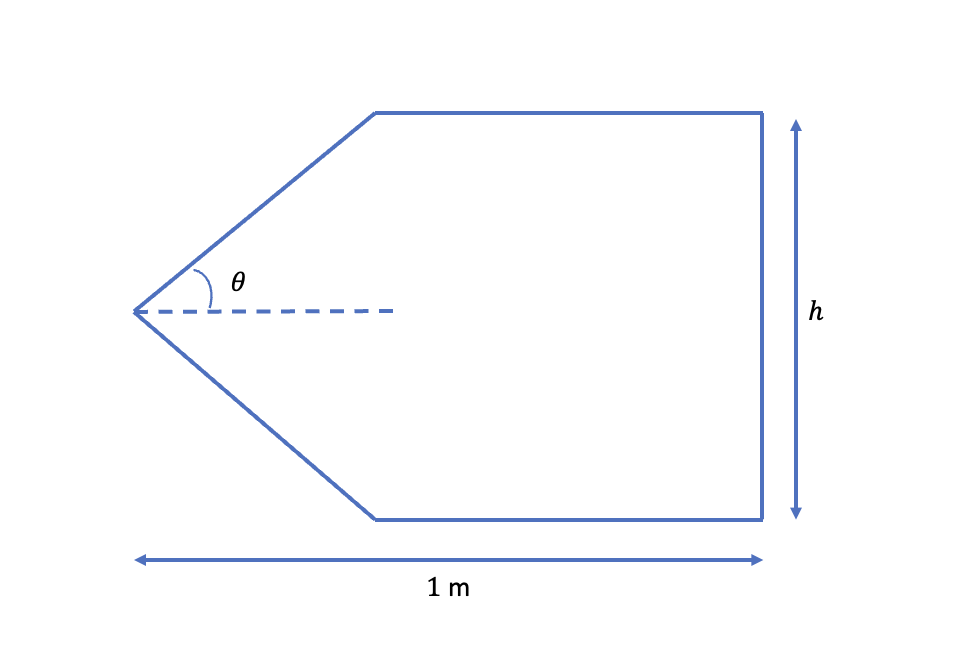
\includegraphics[width=0.5\linewidth]{wedge.png}
    \caption{Triangular wedge profile with the inner half-angle $\theta$ and base height parameter $h$ marked.}
\label{fig:wedge}
\end{figure}


\subsection{Trapezoidal Profile}
The trapezoid is parameterized by the total height $h$ and the flat top length $L_t$, as shown in Equation~\ref{eq:trapezoid_coords}. The lower surface remains fixed at $y = 0$. This geometry produces an inclined leading face followed by a constant-height top surface, as seen in Figure \ref{fig:trapezoid}.
\begin{subequations} \label{eq:trapezoid_coords}
\begin{align}
x &= [0,\; (1 - L_t),\; 1.0] \label{eq:trapezoid_x}\\
y_{\text{top}} &= [0,\; h,\; h] \label{eq:trapezoid_top}\\
y_{\text{bot}} &= [0,\; 0,\; 0] \label{eq:trapezoid_bot}
\end{align}
\end{subequations}
\begin{figure}[H]
\centering
    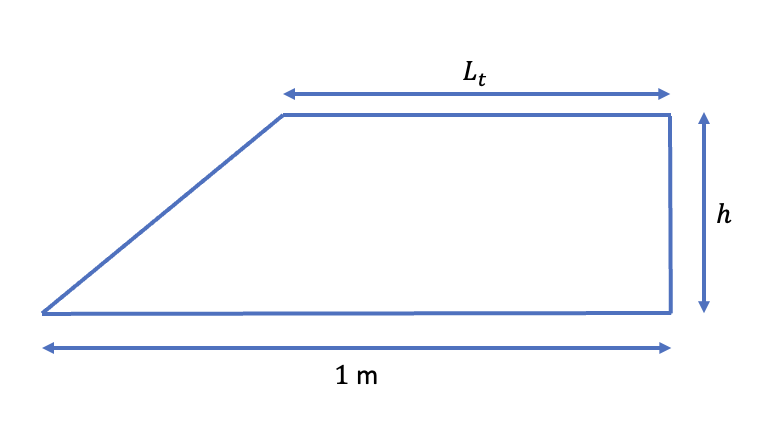
\includegraphics[width=0.5\linewidth]{trapezoid.png}
    \caption{Trapezoidal profile with the base height parameter $h$ and the top length parameter $L_t$ marked.}
\label{fig:trapezoid}
\end{figure}

\subsection{Truncated Diamond Profile}
The diamond-like geometry combines two linear surface segments that meet at an intersection point $(x_i, y_i)$ defined by Equation~\ref{eq:diamond_intersect}. The shape is governed by the base height $h$ and surface slope $m$.
\begin{subequations} \label{eq:diamond_intersect}
\begin{align}
x_i &= \frac{(1+h)/2 - 0.5 + m}{2m} \label{eq:diamond_xi}\\
y_i &= m\,x_i + 0.5 \label{eq:diamond_yi}
\end{align}
\end{subequations}
If the intersection lies within $y_i \le 1$, the result is a sharp, symmetric diamond profile. When $y_i > 1$, the top and bottom surfaces are clipped at the range limits, yielding a truncated (flat-topped) diamond. All diamonds are additionally truncated at the right-hand-side of the bounding box such that they have a non-zero base height. This decision was made in order to ensure that there is enough area at the back end for the nose of the supersonic train to connect to the downstream cars (a diamond ending at a single point, after all, would be very difficult to attach). This decision is also reinforced by the project's regulation that there be two separate points $A$ and $B$ on the right-hand-side of the bounding box. We chose to consider this class of shapes because it can enclose a greater amount of volume while additionally helping to reduce drag via its opposite-orienting faces that will cause pressure drag components to partially cancel out. Figure \ref{fig:diamond} provides an example profile.
\begin{figure}[H]
\centering
    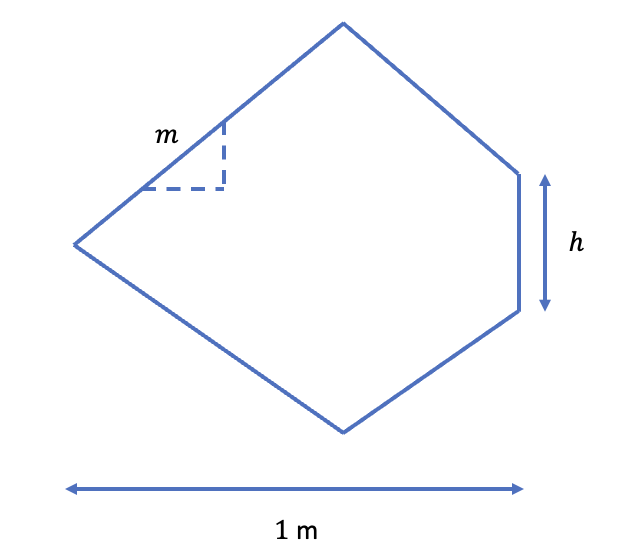
\includegraphics[width=0.5\linewidth]{diamond.png}
    \caption{Truncated diamond profile with the base height parameter $h$ and the slope parameter $m$ marked. Note that if the maximum height of this profile were to exceed $\SI{1}{\meter}$, the top and bottom corners would be clipped to fit the bounding box.}
\label{fig:diamond}
\end{figure}

\section{Results: Inviscid Case} \label{inviscid_results}
\subsection{Parabolic Profiles}
Parabolas were tested for $a \in [0.01, 5]$ and number of points $n \in \left\{3, 4, 5, 6, 10, 20, 50, 100 \right\}$. Figures \ref{fig:inv-parabola-a} and \ref{fig:inv-parabola-b} display, respectively, the cost as it varies over all parabolas generated, as well as the lowest-cost parabolic shape, which achieved a cost of $6.559 \times 10^6$ with $a=0.010$ and $n=10$.
\begin{figure}[H]
\centering
\begin{subfigure}[b]{0.45\textwidth}
    \centering
    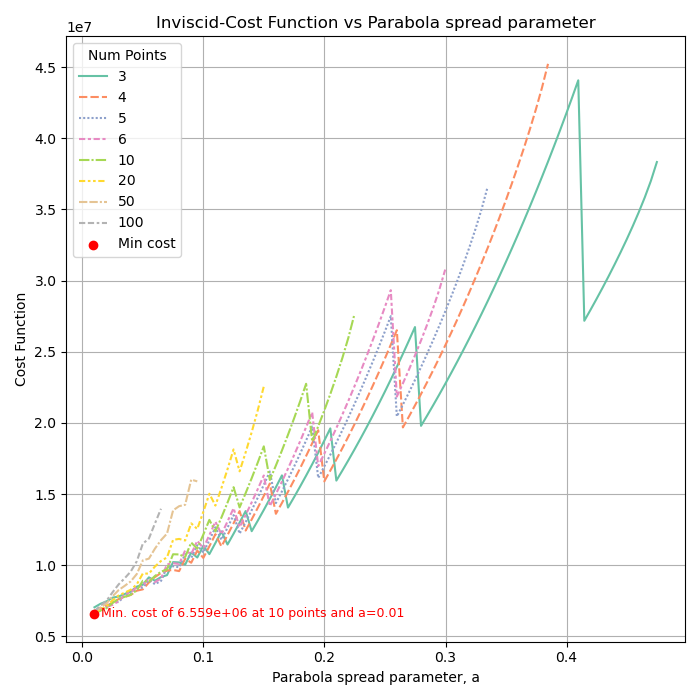
\includegraphics[width=\linewidth]{../results/inviscid/parabolas.png}
    \caption{Inviscid case cost function values plotted over the parabola spread parameter $a$. Separate lines denote the number of points generated per profile. Minimum cost value plotted with red point.}
    \label{fig:inv-parabola-a}
\end{subfigure}
\hfill
\begin{subfigure}[b]{0.45\textwidth}
    \centering
    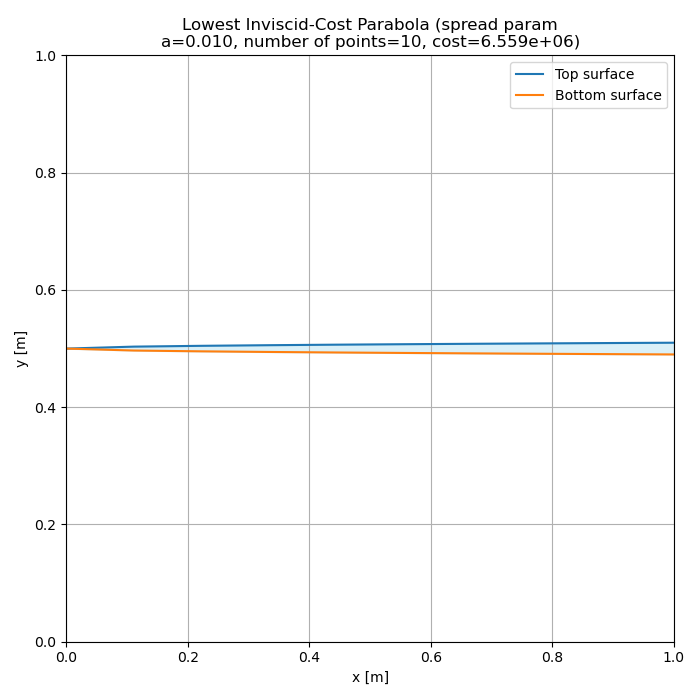
\includegraphics[width=\linewidth]{../results/inviscid/lowest_cost_parabola.png}
    \caption{Profile of the parabola with the smallest inviscid cost function value plotted within the bounding box. Shading between surfaces represents profile's internal area.}
    \label{fig:inv-parabola-b}
\end{subfigure}
\caption{}
\label{fig:inv-parabola}
\end{figure}

\subsection{Power Series Profiles}
The power series profiles were tested for base height values $h \in [0.01, 1] \text{ m}$ and number of points $n \in \left\{3, 5, 10, 20, 50, 100 \right\}$. Figures \ref{fig:inv-power-a} and \ref{fig:inv-power-b} display, respectively, the cost function as it varies over all power series profiles generated, as well as the profile for the lowest-cost power series shape, which achieved a cost of $7.127 \times 10^6$ with $h=0.011 \text{ m}$ and $n=10$.
\begin{figure}[H]
\centering
\begin{subfigure}[b]{0.45\textwidth}
    \centering
    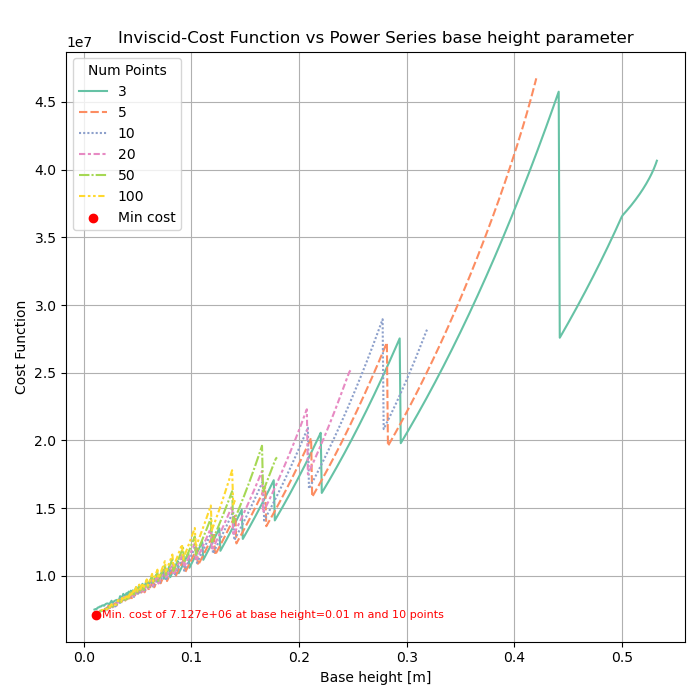
\includegraphics[width=\linewidth]{../results/inviscid/power_series.png}
    \caption{Inviscid case cost function values plotted over the power series base height $h$. Separate lines denote the number of points generated per profile. Minimum cost value plotted with red point.}
    \label{fig:inv-power-a}
\end{subfigure}
\hfill
\begin{subfigure}[b]{0.45\textwidth}
    \centering
    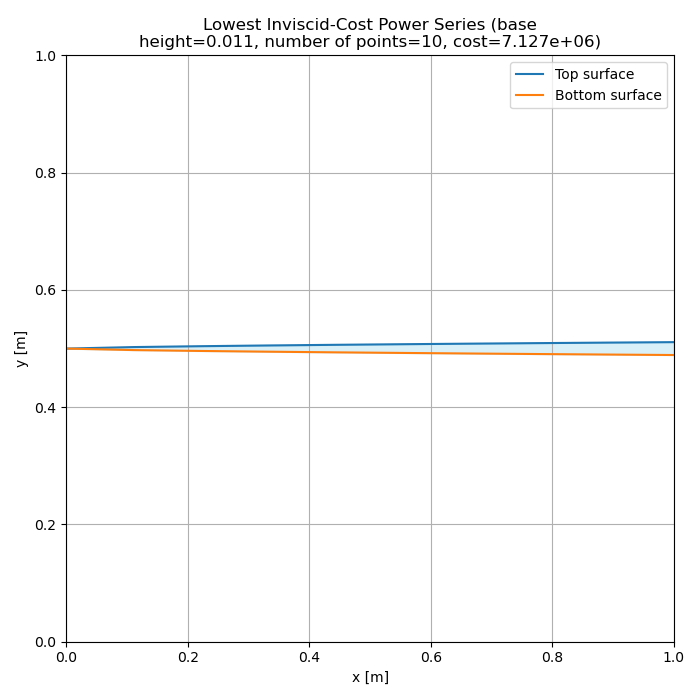
\includegraphics[width=\linewidth]{../results/inviscid/lowest_cost_power_series.png}
    \caption{Profile of the power series shape with the smallest inviscid cost function value plotted within the bounding box. Shading between surfaces represents profile's internal area.}
    \label{fig:inv-power-b}
\end{subfigure}
\caption{}
\label{fig:inv-power}
\end{figure}

\subsection{Triangular Profiles}
The triangular profiles were tested for inner half-angle values of $\theta \in [0.1, 60]\deg$. Figures \ref{fig:inv-triangle-a} and \ref{fig:inv-triangle-b} display, respectively, the cost function as it varies over the parameter of $\theta$, as well as the profile for the lowest-cost triangular profile, which achieved a cost of $8.163 \times 10^6$ with $\theta=0.100\deg$.
\begin{figure}[H]
\centering
\begin{subfigure}[b]{0.45\textwidth}
    \centering
    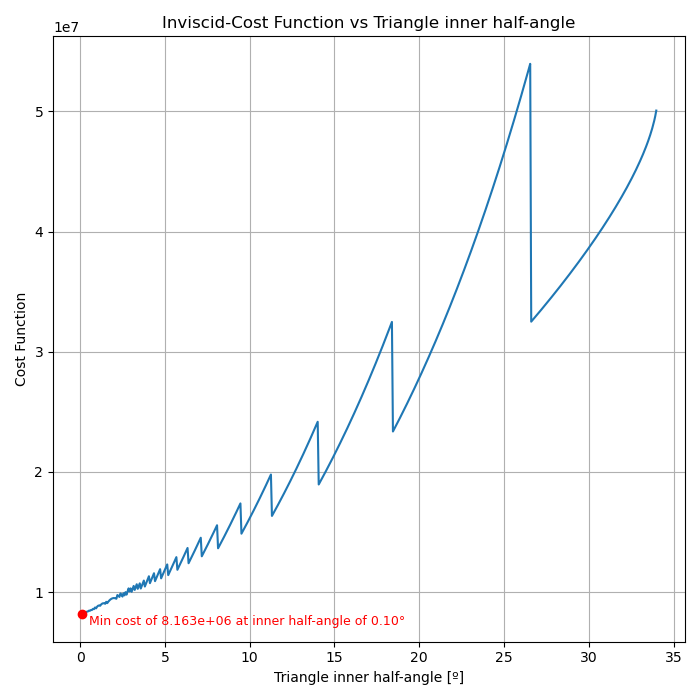
\includegraphics[width=\linewidth]{../results/inviscid/triangles.png}
    \caption{Inviscid cost function plotted versus the triangular inner half-angle $\theta$. Global minimum cost value plotted with red point.}
    \label{fig:inv-triangle-a}
\end{subfigure}
\hfill
\begin{subfigure}[b]{0.45\textwidth}
    \centering
    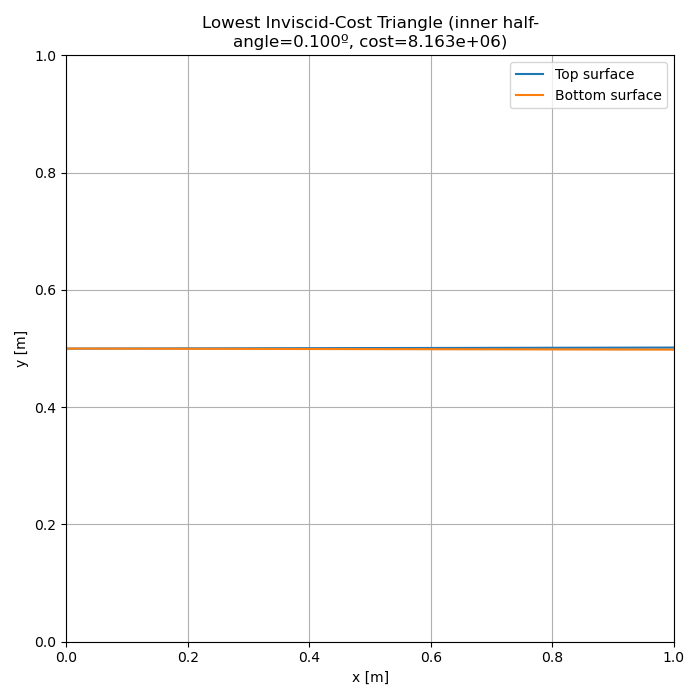
\includegraphics[width=\linewidth]{../results/inviscid/lowest_cost_triangle.png}
    \caption{Triangular profile with the smallest cost function value plotted within the bounding box. Shading between surfaces represents internal area.}
    \label{fig:inv-triangle-b}
\end{subfigure}
\caption{}
\label{fig:inv-triangle}
\end{figure}

\subsection{Triangular Wedge Profiles}
The triangular wedges were tested for inner half-angle values of $\theta \in [0.1, 40]\deg$ and base height values of $h \in [0.01, 0.9]\text{ m}$. Figures \ref{fig:inv-wedge-a} and \ref{fig:inv-wedge-b} display, respectively, the cost function as it varies over both wedge parameters of $\theta$ and $h$, in heat-map form, as well as the profile for the lowest-cost triangular wedge profile, which achieved a cost of $5.043 \times 10^6$ with $h=0.010 \text{ m}$ and $\theta=1.309\deg$.
\begin{figure}[H]
\centering
\begin{subfigure}[b]{0.54\textwidth}
    \centering
    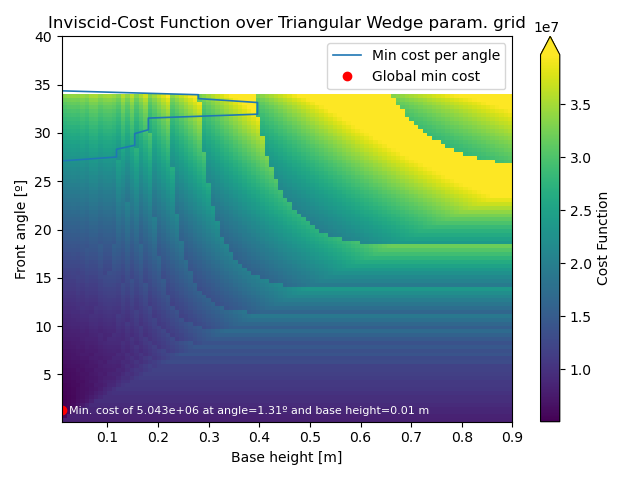
\includegraphics[width=\linewidth]{../results/inviscid/wedges.png}
    \caption{Inviscid case cost function values plotted as a heat map over the triangular wedge inner half-angle $\theta$ and base height $h$. Blue path line denotes the lowest cost achieved per angle. Global minimum cost value plotted with red point.}
    \label{fig:inv-wedge-a}
\end{subfigure}
\hfill
\begin{subfigure}[b]{0.44\textwidth}
    \centering
    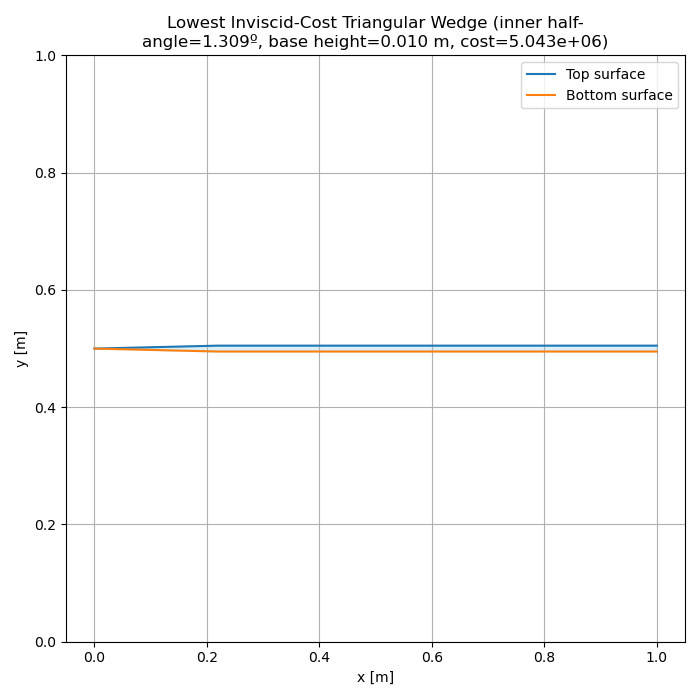
\includegraphics[width=\linewidth]{../results/inviscid/lowest_cost_wedge.png}
    \caption{Profile of the triangular wedge shape with the smallest inviscid cost function value plotted within the bounding box. Shading between surfaces represents internal area.}
    \label{fig:inv-wedge-b}
\end{subfigure}
\caption{}
\label{fig:inv-wedge}
\end{figure}

\subsection{Trapezoidal Profiles}
The trapezoidal profiles were tested for height values of $h \in [0.01, 0.7]\text{ m}$ and top length values of $L_t \in [0.1, 0.9]\text{ m}$. Figures \ref{fig:inv-trapezoid-a} and \ref{fig:inv-trapezoid-b} display, respectively, the cost function as it varies over the parameters of $h$ and $L_t$, in heat-map form, as well as the profile for the lowest-cost trapezoidal profile, which achieved a cost of $5.498\times 10^6$ with $h=0.010 \text{ m}$ and $L_t=0.755 \text{ m}$.
\begin{figure}[H]
\centering
\begin{subfigure}[b]{0.54\textwidth}
    \centering
    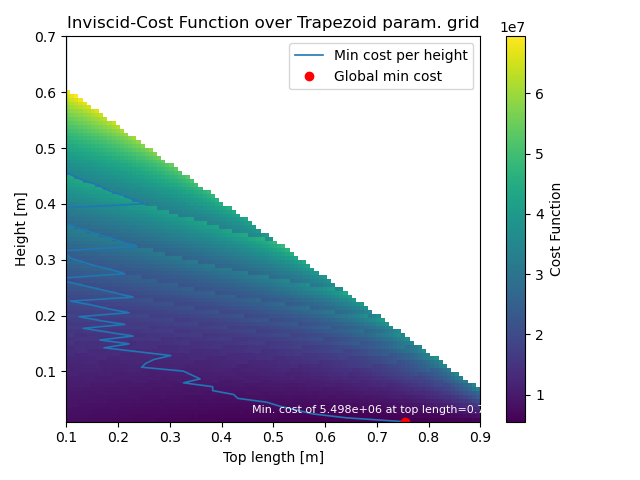
\includegraphics[width=\linewidth]{../results/inviscid/trapezoids.png}
    \caption{Inviscid case cost function values plotted as a heat map over the trapezoid height $h$ and top length $L_t$. Blue path line denotes the lowest cost achieved per top length value. Global minimum cost value plotted with red point.}
    \label{fig:inv-trapezoid-a}
\end{subfigure}
\hfill
\begin{subfigure}[b]{0.44\textwidth}
    \centering
    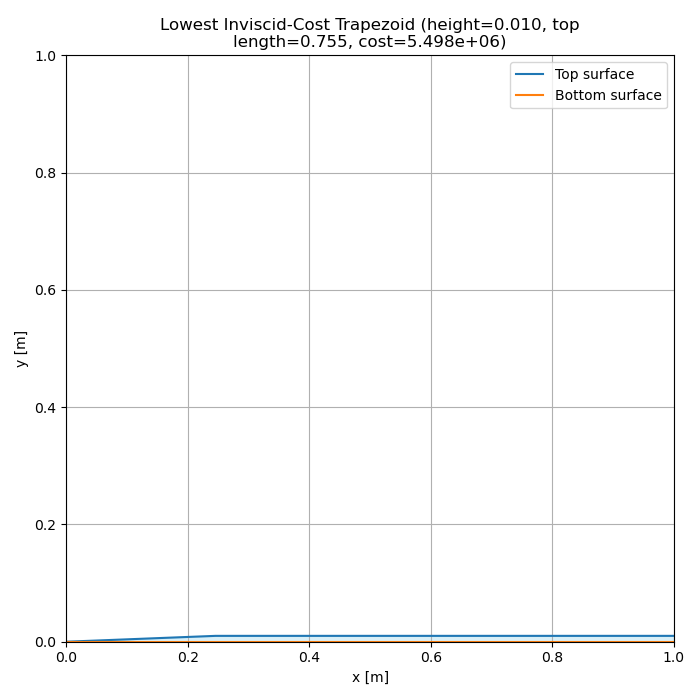
\includegraphics[width=\linewidth]{../results/inviscid/lowest_cost_trapezoid.png}
    \caption{Profile of the trapezoidal shape with the smallest inviscid cost function value plotted within the bounding box. Shading between surfaces represents internal area.}
    \label{fig:inv-trapezoid-b}
\end{subfigure}
\caption{}
\label{fig:inv-trapezoid}
\end{figure}

\subsection{Truncated Diamond Profiles}
The truncated diamond profiles were tested for base height values of $h \in [0.01, 1.0]\text{ m}$ and slope values of $m \in [0.1, 0.75]$. Figures \ref{fig:inv-diamond-a} and \ref{fig:inv-diamond-b} display, respectively, the cost function as it varies over both parameters of $h$ and $m$, in heat-map form, as well as the profile for the lowest-cost diamond profile, which achieved a cost of $7.466\times 10^6$ with $h=0.020 \text{ m}$ and $m=0.100$.
\begin{figure}[H]
\centering
\begin{subfigure}[b]{0.54\textwidth}
    \centering
    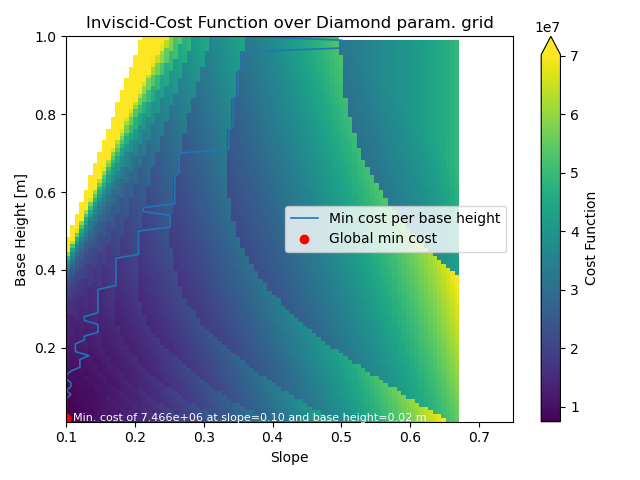
\includegraphics[width=\linewidth]{../results/inviscid/diamonds.png}
    \caption{Inviscid case cost function values plotted as a heat map over the diamond base height $h$ and slope $m$. Blue path line denotes the lowest cost achieved per base height value. Global minimum cost value plotted with red point.}
    \label{fig:inv-diamond-a}
\end{subfigure}
\hfill
\begin{subfigure}[b]{0.44\textwidth}
    \centering
    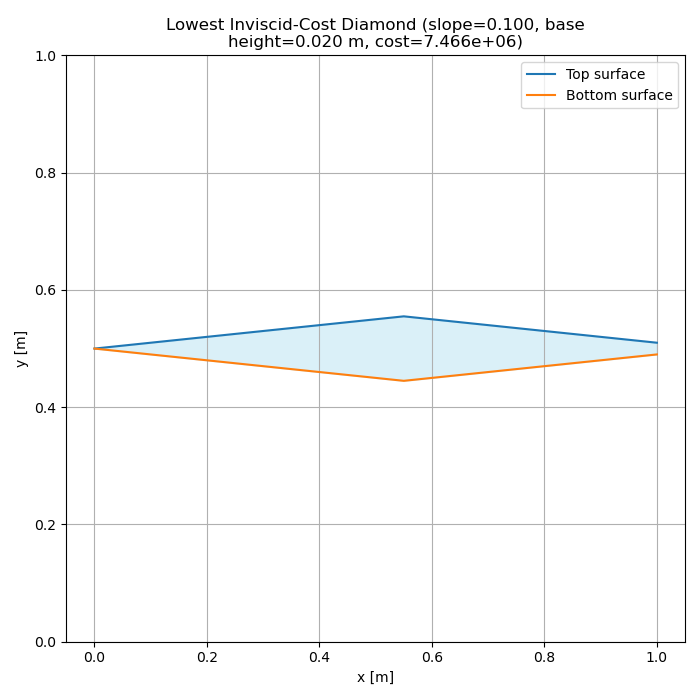
\includegraphics[width=\linewidth]{../results/inviscid/lowest_cost_diamond.png}
    \caption{Profile of the diamond shape with the smallest inviscid cost function value plotted within the bounding box. Shading between surfaces represents internal area.}
    \label{fig:inv-diamond-b}
\end{subfigure}
\caption{}
\label{fig:inv-diamond}
\end{figure}


\section{Results: Viscous Case} \label{viscous_results}
For the viscous physical model, all profiles were tested acros the same parameter space as described in Section \ref{inviscid_results}.
\subsection{Parabolic Profiles}
 Figures \ref{fig:vis-parabola-a} and \ref{fig:vis-parabola-b} display, respectively, the cost as it varies over all parabolas generated, as well as the lowest-cost parabolic shape, which achieved a cost of $1.525 \times 10^7$ with $a=0.100$ and $n=4$.
\begin{figure}[H]
\centering
\begin{subfigure}[b]{0.45\textwidth}
    \centering
    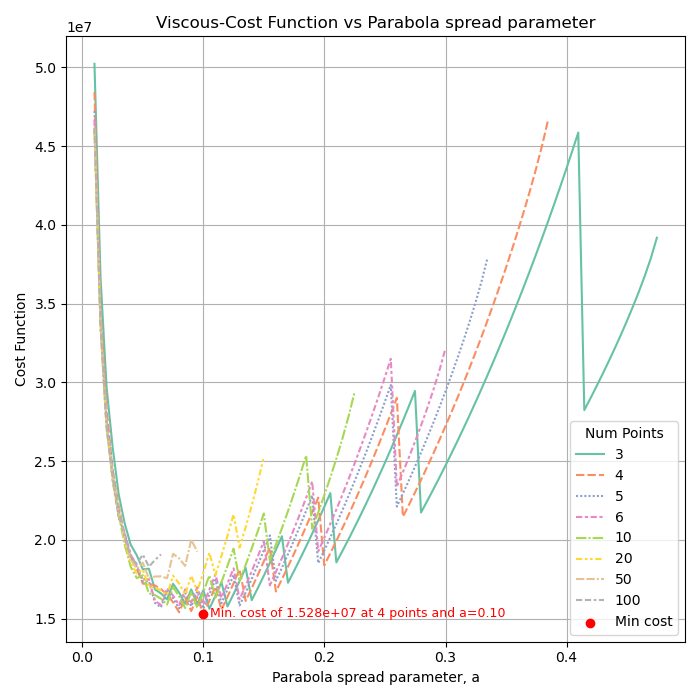
\includegraphics[width=\linewidth]{../results/viscous/parabolas.png}
    \caption{Viscous case cost function values plotted over the parabola spread parameter $a$. Separate lines denote the number of points generated per profile. Minimum cost value plotted with red point.}
    \label{fig:vis-parabola-a}
\end{subfigure}
\hfill
\begin{subfigure}[b]{0.45\textwidth}
    \centering
    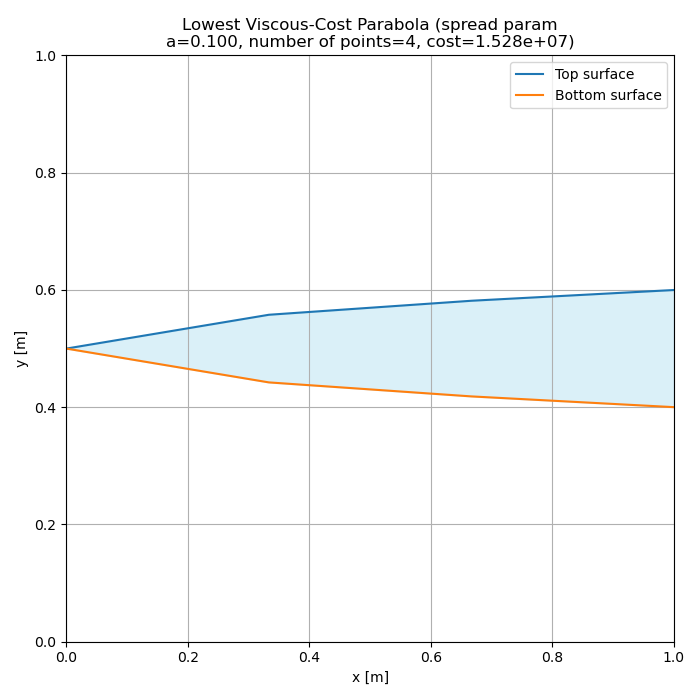
\includegraphics[width=\linewidth]{../results/viscous/lowest_cost_parabola.png}
    \caption{Profile of the parabola with the smallest viscous cost function value plotted within the bounding box. Shading between surfaces represents profile's internal area.}
    \label{fig:vis-parabola-b}
\end{subfigure}
\caption{}
\label{fig:vis-parabola}
\end{figure}

\subsection{Power Series Profiles}
Figures \ref{fig:vis-power-a} and \ref{fig:vis-power-b} display, respectively, the cost function as it varies over all power series profiles generated, as well as the profile for the lowest-cost power series shape, which achieved a cost of $1.558 \times 10^7$ with $h=0.106 \text{ m}$ and $n=5$.
\begin{figure}[H]
\centering
\begin{subfigure}[b]{0.45\textwidth}
    \centering
    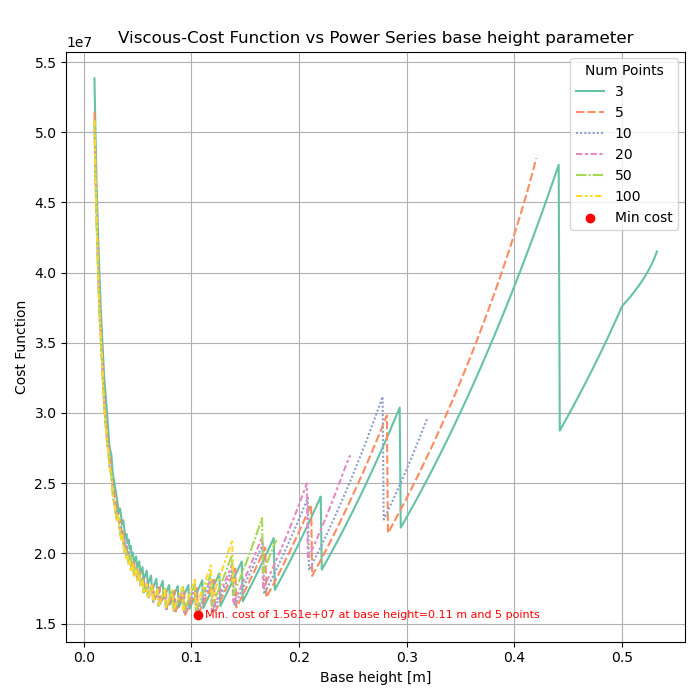
\includegraphics[width=\linewidth]{../results/viscous/power_series.png}
    \caption{Viscous case cost function values plotted over the power series base height $h$. Separate lines denote the number of points generated per profile. Minimum cost value plotted with red point.}
    \label{fig:vis-power-a}
\end{subfigure}
\hfill
\begin{subfigure}[b]{0.45\textwidth}
    \centering
    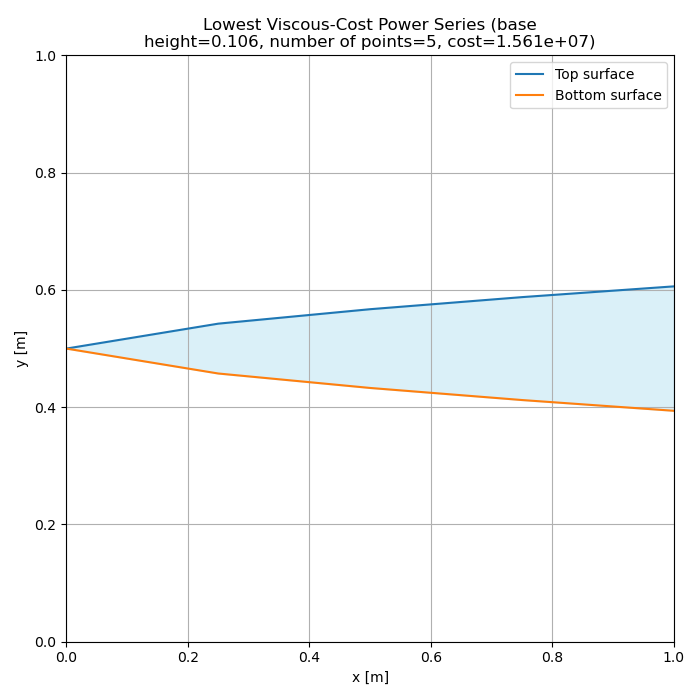
\includegraphics[width=\linewidth]{../results/viscous/lowest_cost_power_series.png}
    \caption{Profile of the power series shape with the smallest viscous cost function value plotted within the bounding box. Shading between surfaces represents profile's internal area.}
    \label{fig:vis-power-b}
\end{subfigure}
\caption{}
\label{fig:vis-power}
\end{figure}

\subsection{Triangular Profiles}
Figures \ref{fig:vis-triangle-a} and \ref{fig:vis-triangle-b} display, respectively, the cost function as it varies over $\theta$, as well as the profile for the lowest-cost triangular profile, which achieved a cost of $1.794 \times 10^7$ with $\theta=5.736\deg$.
\begin{figure}[H]
\centering
\begin{subfigure}[b]{0.45\textwidth}
    \centering
    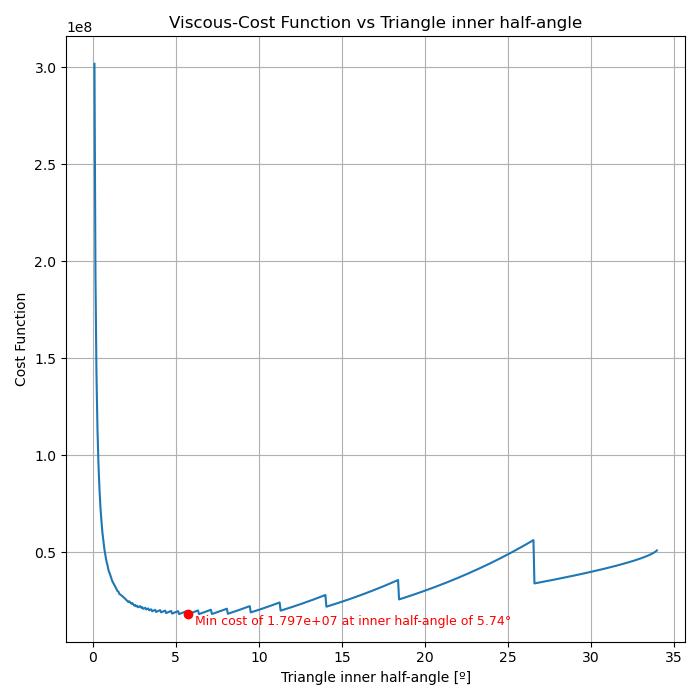
\includegraphics[width=\linewidth]{../results/viscous/triangles.png}
    \caption{Viscous cost function plotted versus the triangular inner half-angle $\theta$. Global minimum cost value plotted with red point.}
    \label{fig:vis-triangle-a}
\end{subfigure}
\hfill
\begin{subfigure}[b]{0.45\textwidth}
    \centering
    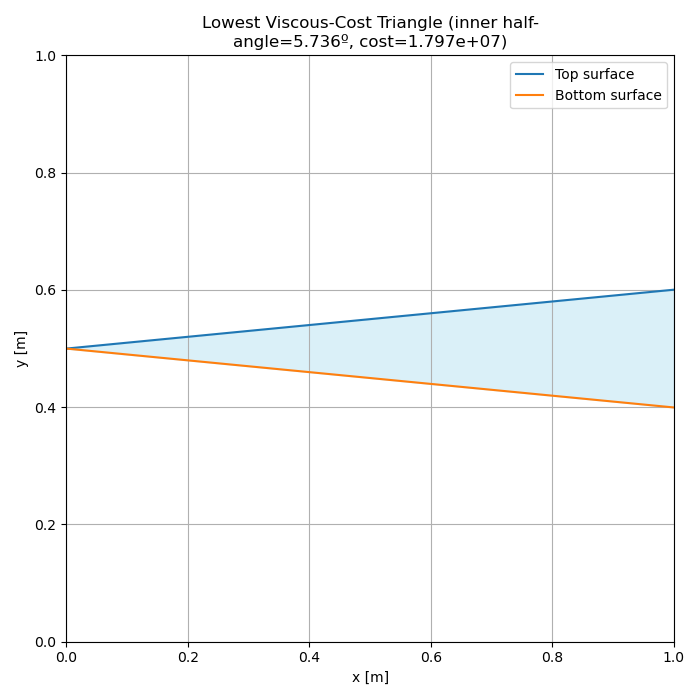
\includegraphics[width=\linewidth]{../results/viscous/lowest_cost_triangle.png}
    \caption{Triangular profile with the smallest cost function value plotted within the bounding box. Shading between surfaces represents internal area.}
    \label{fig:vis-triangle-b}
\end{subfigure}
\caption{}
\label{fig:vis-triangle}
\end{figure}

\subsection{Triangular Wedge Profiles}
Figures \ref{fig:vis-wedge-a} and \ref{fig:vis-wedge-b} display, respectively, the cost function as it varies over both wedge parameters of $\theta$ and $h$, in heat-map form, as well as the profile for the lowest-cost triangular wedge profile, which achieved a cost of $1.464 \times 10^7$ with $h=0.136 \text{ m}$ and $\theta=7.355\deg$.
\begin{figure}[H]
\centering
\begin{subfigure}[b]{0.54\textwidth}
    \centering
    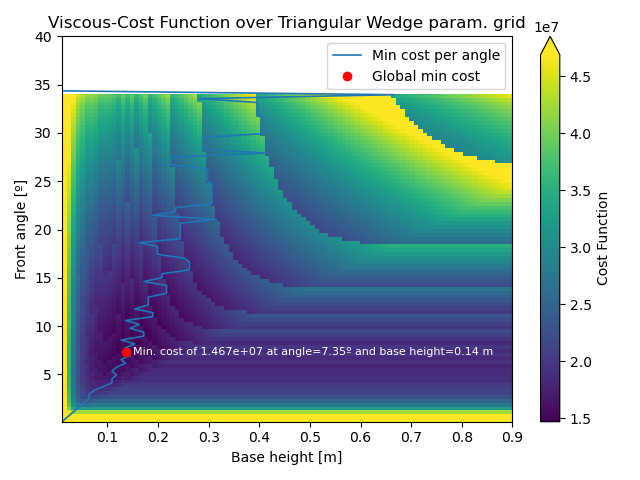
\includegraphics[width=\linewidth]{../results/viscous/wedges.png}
    \caption{Viscous case cost function values plotted as a heat map over the triangular wedge inner half-angle $\theta$ and base height $h$. Blue path line denotes the lowest cost achieved per angle. Global minimum cost value plotted with red point.}
    \label{fig:vis-wedge-a}
\end{subfigure}
\hfill
\begin{subfigure}[b]{0.44\textwidth}
    \centering
    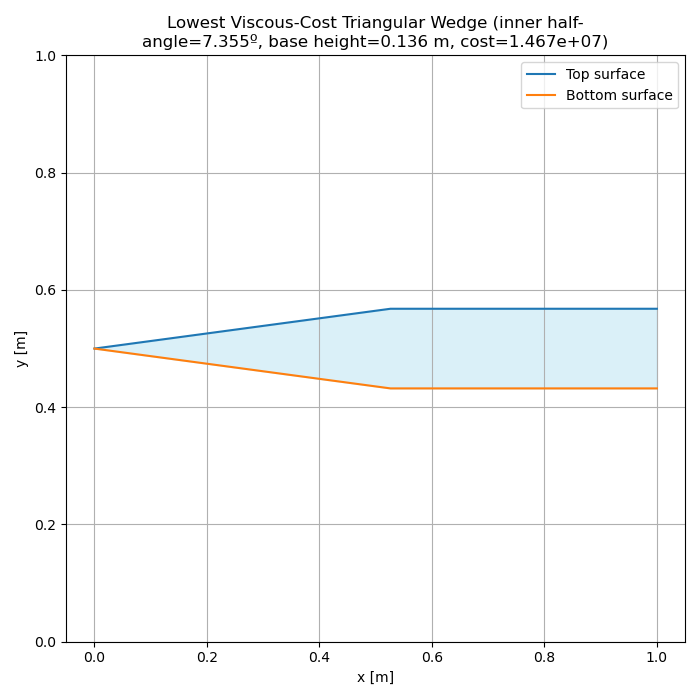
\includegraphics[width=\linewidth]{../results/viscous/lowest_cost_wedge.png}
    \caption{Profile of the triangular wedge shape with the smallest viscous cost function value plotted within the bounding box. Shading between surfaces represents internal area.}
    \label{fig:vis-wedge-b}
\end{subfigure}
\caption{}
\label{fig:vis-wedge}
\end{figure}

\subsection{Trapezoidal Profiles}
Figures \ref{fig:vis-trapezoid-a} and \ref{fig:vis-trapezoid-b} display, respectively, the cost function as it varies over the parameters of $h$ and $L_t$, in heat-map form, as well as the profile for the lowest-cost trapezoidal profile, which achieved a cost of $1.893\times 10^7$ with $h=0.100 \text{ m}$ and $L_t=0.431 \text{ m}$.
\begin{figure}[H]
\centering
\begin{subfigure}[b]{0.54\textwidth}
    \centering
    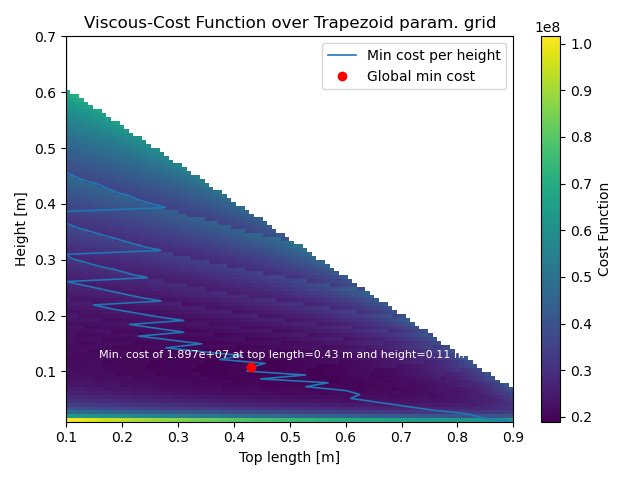
\includegraphics[width=\linewidth]{../results/viscous/trapezoids.png}
    \caption{Viscous case cost function values plotted as a heat map over the trapezoid height $h$ and top length $L_t$. Blue path line denotes the lowest cost achieved per top length value. Global minimum cost value plotted with red point.}
    \label{fig:vis-trapezoid-a}
\end{subfigure}
\hfill
\begin{subfigure}[b]{0.44\textwidth}
    \centering
    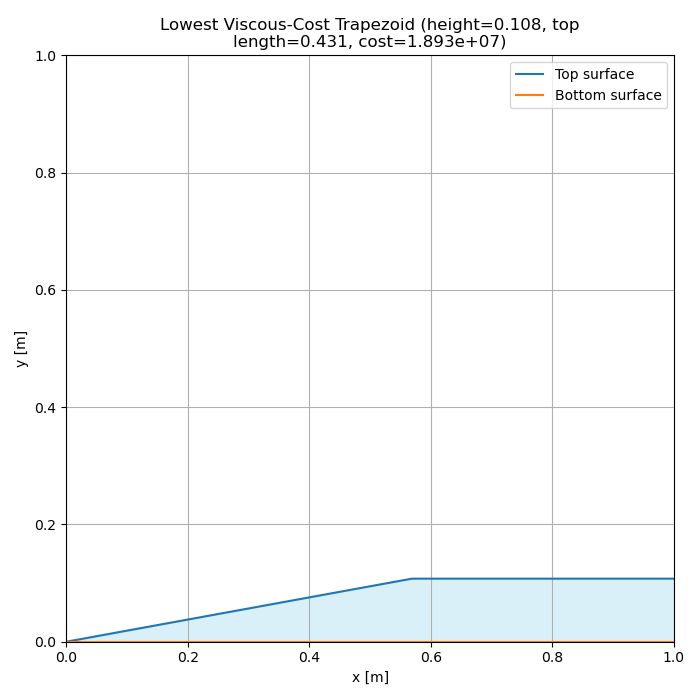
\includegraphics[width=\linewidth]{../results/viscous/lowest_cost_trapezoid.png}
    \caption{Profile of the trapezoidal shape with the smallest viscous cost function value plotted within the bounding box. Shading between surfaces represents internal area.}
    \label{fig:vis-trapezoid-b}
\end{subfigure}
\caption{}
\label{fig:vis-trapezoid}
\end{figure}

\subsection{Truncated Diamond Profiles}
Figures \ref{fig:vis-diamond-a} and \ref{fig:vis-diamond-b} display, respectively, the cost function as it varies over both parameters of $h$ and $m$, in heat-map form, as well as the profile for the lowest-cost diamond profile, which achieved a cost of $1.491\times 10^7$ with $h=0.090 \text{ m}$ and $m=0.126$.
\begin{figure}[H]
\centering
\begin{subfigure}[b]{0.54\textwidth}
    \centering
    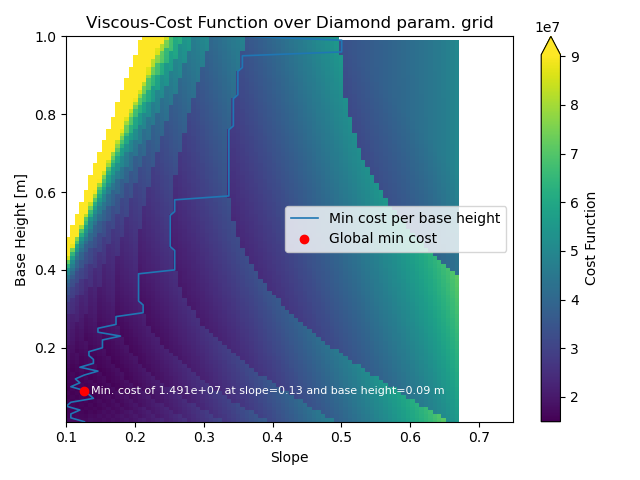
\includegraphics[width=\linewidth]{../results/viscous/diamonds.png}
    \caption{Viscous case cost function values plotted as a heat map over the diamond base height $h$ and slope $m$. Blue path line denotes the lowest cost achieved per base height value. Global minimum cost value plotted with red point.}
    \label{fig:vis-diamond-a}
\end{subfigure}
\hfill
\begin{subfigure}[b]{0.44\textwidth}
    \centering
    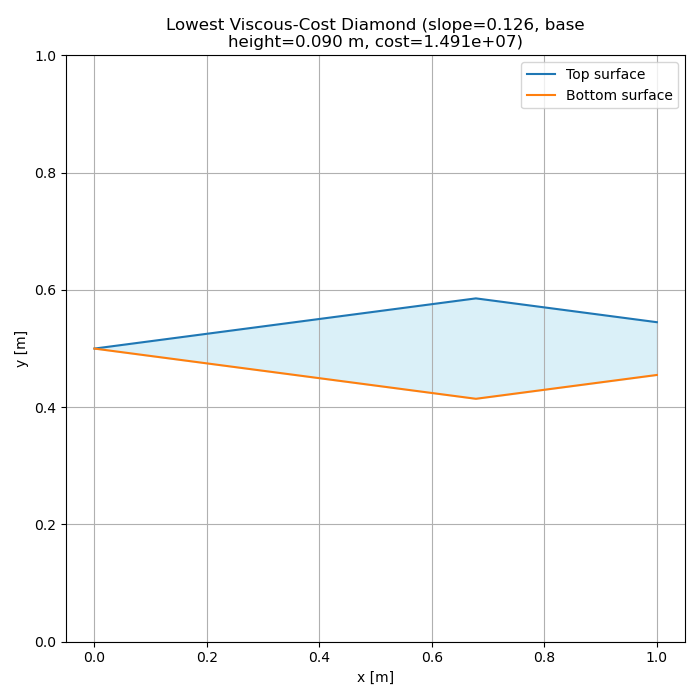
\includegraphics[width=\linewidth]{../results/viscous/lowest_cost_diamond.png}
    \caption{Profile of the diamond shape with the smallest viscous cost function value plotted within the bounding box. Shading between surfaces represents internal area.}
    \label{fig:vis-diamond-b}
\end{subfigure}
\caption{}
\label{fig:vis-diamond}
\end{figure}

\section{Discussion}
After generating all profiles and evaluating their cost functions, we compared and found the overall lowest-cost shape across all classes for each case (inviscid and viscous).

From Section \ref{inviscid_results}, we see that \textbf{the optimal shape for the inviscid case is a triangular wedge of height $\mathbf{0.01}$ m and angle $\mathbf{1.309}$º with a cost of $\mathbf{5.043 \times 10^6}$}. The profile of this shape can be seen in Figure \ref{fig:inv-wedge-b}.

From Section \ref{viscous_results}, we see that \textbf{the optimal shape for the viscous case is a triangular wedge of height $\mathbf{0.136}$ m and angle $\mathbf{7.355}$º with a cost of $\mathbf{1.464 \times 10^7}$}. The profile of this shape can be seen in Figure \ref{fig:vis-wedge-b}.

As expected, the lowest cost for the viscous model is higher than that of the inviscid model, due to the addition of skin drag on all surfaces.

For both cases, it can be seen that all plots of the cost function over the parameter space display a somewhat oscillatory behavior of vertical jumps (in 2D plots) and sharp cliffs (in 3D plots). This comes directly from the trip-count formula in Eq. \ref{eq:num_trips}, which uses a ceiling to enforce integer trips. As the enclosed area changes continuously, $N$ stays flat until the ratio in \ref{eq:num_trips} crosses the next integer threshold; at that point $N$ jumps by 2 (outbound and return). Those discontinuities propagate into the overall cost function as well, and are displayed in the graph.

Across all shape classes, it should be noted that the lowest-cost inviscid shapes are much thinner than their viscous counterparts. In fact, almost all of the optimal shapes for the inviscid case have parameters that result in the minimum thickness (with almost zero volume). This is because in a physical model with no skin friction, drag's role in the cost function will dominate, since it is very possible to drive pressure drag down to zero, whereas the number of trips within the cost function is limited to be at least one. Thus, whatever shape is thinnest will always have the least drag (since most pressure will be normal to the incoming flow), which drives the cost function to zero (even as the number of trips increase).

In contrast, the viscous case favors shapes that have a thicker profile that encloses more area. This is because in a physical model with friction, skin drag acts upon the shape regardless of how thin it is, and we therefore cannot simply drive thickness to zero. Skin friction adds a term proportional to local dynamic pressure and wetted area, so making the profile longer or adding curvature increases the skin drag. At the same time, enclosing more area reduces $N$. The optimum is the balance point where the marginal increase in skin friction is offset by the marginal decrease in trips. That is why the viscous winners are thicker and enclose more area than the inviscid winners.

It is interesting that both cases favor the triangular wedge. This is likely because the back portion of the triangular wedge, which is comprised of two horizontal segments, greatly increase enclosed area without increasing any drag for the inviscid case, and only slightly increasing skin drag for the viscous case. As previously mentioned is the trend for all shapes, the wedge for the viscous case is thicker than that of the inviscid case.

It was noted throughout this process that generally, shapes with a lower resolution (such as lower resolution parabolas and power series, or fixed low-resolution polygons) were favored. I believe that this is because a series of many small oblique shocks will preserve more static pressure across the shape, as seen in the results of Homework 3, whereas a smaller number of larger-angled oblique shocks will cause more pressure loss, which will then decrease drag. Additionally, coarser discretizations reduce total wetted length for a given non-polygonal shape, which lowers viscous drag (though it should be noted that the effects of this would be quite minimal in comparison to other effects).

One limitation of our design process is the assumption of 1D flow and of constant profile into the depth of the bounding box. Real nose cones are three-dimensional, and will have variable geometry into the depth of the page, and so will provide different (and perhaps better) results. I note that these results may be better because if we do not include curvature in the third dimension, we are increasing the amount of planar surfaces normal to the incoming flow, and therefore increasing drag. Additionally, real flow conditions across the surfaces will experience detached shocks, as well as shock-shock interactions, both of which are ignored in our analysis, and provide more complexity to the profiles we optimize. A full computational fluid dynamics (CFD) analysis may be appropriate to capture the full extent of this behavior. For the viscous drag model as well, we assumed a constant drag coefficient of $C_D = 0.01$ for all surfaces, though real-life behavior would likely cause skin friction to depend on the Reynolds Number, the Mach Number, and other variable flow conditions. Additionally, the cost function we are provided with is quite limited: there are no penalties or rewards for manufacturability, heating effects, and partial loading of the train. Finally, we made an assumption that the $AB$ back-face pressure is set to zero. This idealizes the real boundary, but real-life conditions would likely have non-zero pressure that affect drag (and perhaps actually decrease drag, due to the direction that the pressure acts).

\section{Conclusion}
Within the assignment constraints, triangular wedges provide the best trade between drag and trip count in both models, with thicker wedges preferred when skin friction is included. The report includes comparisons of cost functions across families of shapes, drag calculations, and a discussion of inviscid vs. viscous differences and analysis limits.

\printbibliography


\end{document}